\documentclass[french]{article}
\usepackage[T1]{fontenc}
\usepackage[utf8]{inputenc}
\usepackage{lmodern}
\usepackage[a4paper]{geometry}
\usepackage{babel}
\usepackage{float}
\usepackage{graphicx}
\begin{document}

\section{synthèse d'un filtre passe-bande}

La synthèse d'un filtre en hautes fréquences à partir d'un gabarit se rapporte à la méthode étudiée en moyenne fréquence. Une étape finale est ajoutée permettant la transformation des éléments localisés en éléments distribués.
Le cahier des charges est le suivant, concevoir un filtre passe bande basé sur une fonction d'approximation de type Tchebychev et respectant le gabarit figure \ref{fig:gab}. L'implémentation réelle doit se en utilisant exclusivement des lignes micro ruban de longueur $\frac{\lambda_g}{2}$ ou $\frac{\lambda_g}{4}$ et des stubs.

\begin{figure}[H]
	\centering
	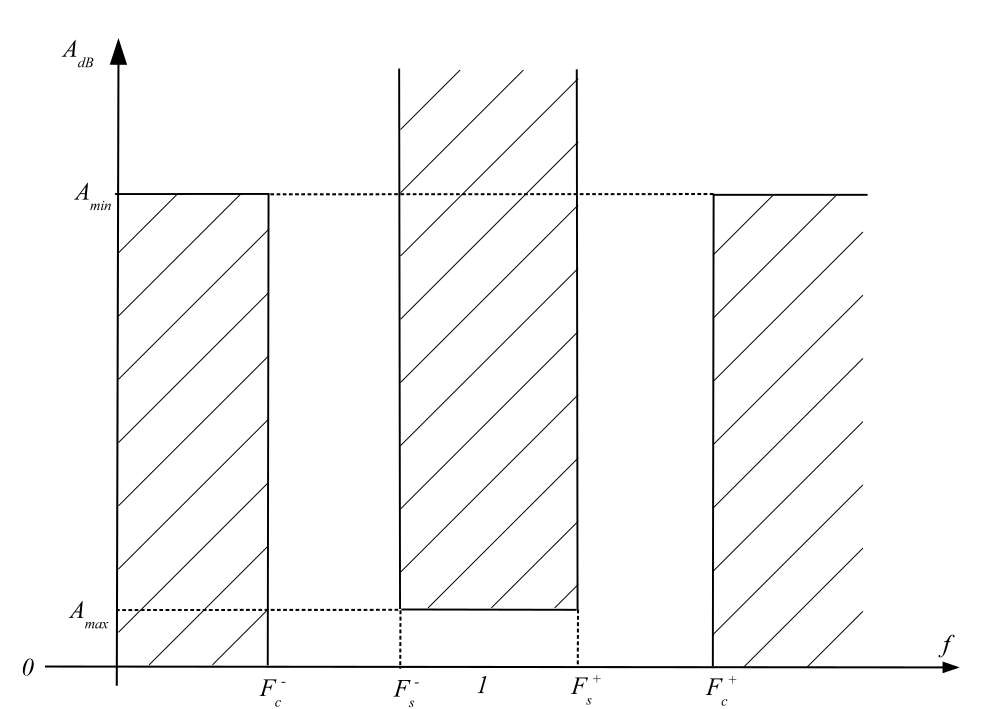
\includegraphics[width=0.5\linewidth]{ressources/gabarit_passe_bande}
	\caption{Gabarit du filtre passe-bas souhaité}
	\label{fig:gab}
\end{figure}
Les valeurs numériques associées au gabarit sont les suivantes. Les fréquences sont en GHz et l'atténuation en dB. 
	\begin{table}[H]
		\centering
\begin{tabular}{|c|c|c|c|c|c|}
		\hline
	$A_{max}$& $A_{min}$ & $f_c^-$ & $f_s^-$ & $f_s^+$ &$f_c^+$ \\ \hline
	0,1000	 & 15,00 		& 1,500	   & 1,750 & 2,250& 3,000 \\ \hline
	\end{tabular}
\caption{Valeur numérique gabarit souhaité}
	\end{table}
\paragraph{Symétrie du gabarit} ~~\\ \noindent
Avant de commencer la synthèse du filtre il faut valider une condition sur la symétrie. Si elle n'est pas respectée il faut modifier le gabarit du cahier des charges. La condition s'opère sur la moyenne géométrique de la bande passante et de la bande coupée.
\begin{equation}
	 f_{co} = \sqrt{f_c^-.f_c^+}, \quad f_{so} = \sqrt{f_s^- f_s^+}
\end{equation}
Ainsi, si $f_{so} = f_{co}$, le gabarit est centré il n'est pas nécessaire de réaliser d'opération particulaire. On obtient a alors  $f_{so} = f_{co} = f_0$ avec $f_0$ la fréquence centrale du gabarit. Si $f_{so} \neq f_{co}$, le gabarit n'est pas centré il faut passer par une étape de centrage du gabarit avant de réaliser la synthèse du filtre.\\
Application numérique :\\
\begin{equation}
f_{co} = \sqrt{f_c^-.f_c^+} = \sqrt{1,500*3,000} = 2,121 GHz
\end{equation}
\begin{equation}
	f_{so} = \sqrt{f_s^- f_s^+} = \sqrt{1,750*2,250} = 1,984 GHz
\end{equation}
\begin{equation}
f_{so} <	f_{co}
\end{equation}
Le filtre est asymétrique il faut réaliser l'opération de centrage. Dans notre cas elle vise à diminuer $f_{co}$. Il n'est possible de faire varier que la borne positive $.f_c^+$. Cela à pour effet de sur contraindre le cahier des charges. Pour répondre aux exigences il est interdit d'élargir la bande atténué ou de diminuer la bande passante. \footnote{Il existe une méthode détaillée dans le \textit{cours de filtrage actif} de Vincent Gouret faisant varier à la fois $f_{so}$ et $f_{co}$. Elle permet d'optimiser la contrainte sur le sélectivité. Dans notre cas cela ne change pas l'ordre du filtre.}
Il vient donc :
\begin{equation}
f_c^+=\frac{f_{so}^2}{f_c^-}=\frac{1,984^2}{1,500}=2,614GHz
\end{equation}
Les nouvelles valeurs numériques pour le gabarit du filtre sont les suivantes. Elle font référence à la figure \ref{fig:gab}.
	\begin{table}[H]
	\centering
	\begin{tabular}{|c|c|c|c|c|c|}
		\hline
		$A_{max}$& $A_{min}$ & $f_c^-$ & $f_s^-$ & $f_s^+$ &$f_c^+$ \\ \hline
		0,100		 & 15,00 		& 1,500	   & 1,75 & 2,250& 2,614 \\ \hline
	\end{tabular}
	\caption{Valeur numérique gabarit centré}
\end{table}
\paragraph{Gabarit passe bas} ~~\\ \noindent
L'étape suivant dans la conception d'un filtre passe bande symétrique vise à simplifier la synthèse en passant par un gabarit passe bas. Cela permet de calculer son ordre puis sa structure en éléments localisés.
\begin{figure}[H]
	\centering
	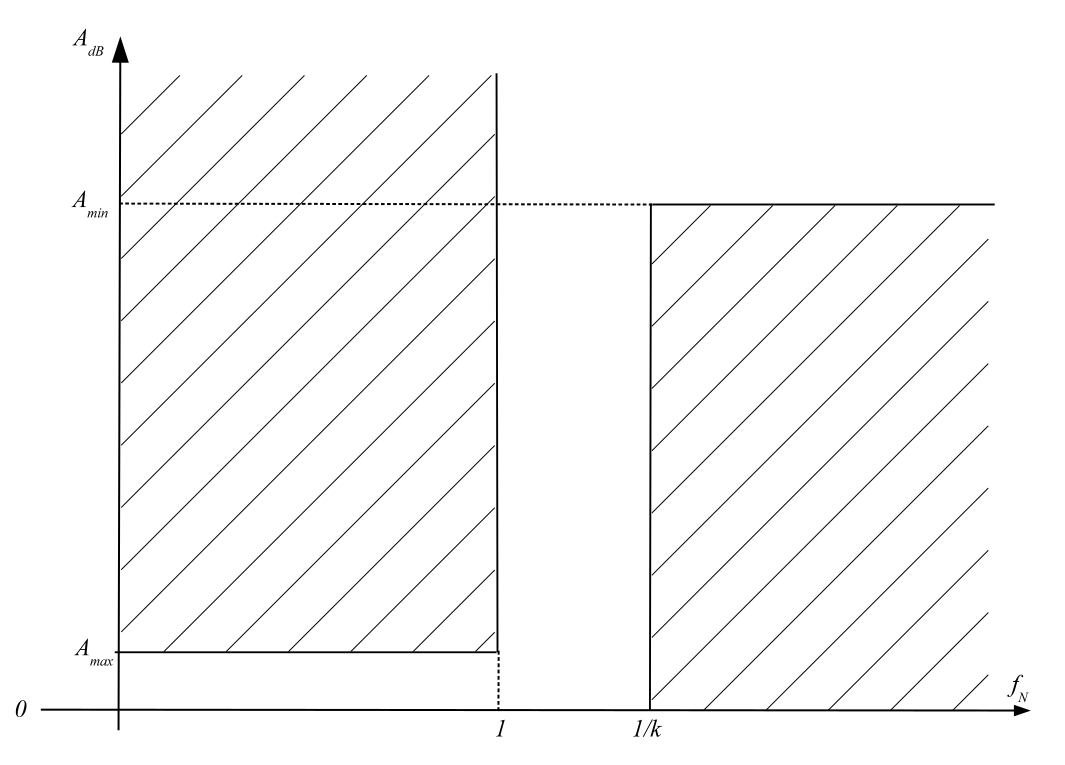
\includegraphics[width=0.5\linewidth]{ressources/gabarit_passe_pas}
	\caption{Gabarit filtre passe bas équivalent}
	\label{fig:gabaritpassepas}
\end{figure}
L'évaluation du coefficient de sélectivité permet d'établir le gabarit normalisée. Cette grandeur se note $k$ est sans unité et strictement inférieure à 1. Son expression est la suivante :
\begin{equation}
	k=\frac{\Delta.f_s}{\Delta.f_c}=\frac{f_s^+-f_s^-}{f_c^+-f_c^-}=\frac{2,250-1,75}{2,614-1,500}=
\end{equation}
\end{document}
